%%%%%%%%%%%%%%%%%%%%%%%%%%%%%%%%%%%%%%%%%%%%%%%%%%%%%%%%%%%%%%%%%%%%%%%%%%%%%%%%
% operation.tex: Chapter on Detector Operation and Performance:
%%%%%%%%%%%%%%%%%%%%%%%%%%%%%%%%%%%%%%%%%%%%%%%%%%%%%%%%%%%%%%%%%%%%%%%%%%%%%%%%
\chapter{Detector Operation}
\label{operation_chapter}
%%%%%%%%%%%%%%%%%%%%%%%%%%%%%%%%%%%%%%%%%%%%%%%%%%%%%%%%%%%%%%%%%%%%%%%%%%%%%%%%

%%%%%%%%%%%%%%%%%%%%%%%%%%%%%%%%%%%%%%%%%%%%%%%%%%%%%%%%%%%%%%%%%%%%%%%%%%%%%%%%
% Detector Yield 
%%%%%%%%%%%%%%%%%%%%%%%%%%%%%%%%%%%%%%%%%%%%%%%%%%%%%%%%%%%%%%%%%%%%%%%%%%%%%%%%
\section{Detector Yield}
\label{sec:yield}
%%%%%%%%%%%%%%%%%%%%%%%%%%%%%%%%%%%%%%%%%%%%%%%%%%%%%%%%%%%%%%%%%%%%%%%%%%%%%%%%

You need to say \ac{EBEX} and \ac{SQUID} before the table ...

\begin{table}[ht!]
\begin{center}
\begin{tabular}{l|c|c|c|c}
  & 150~GHz & 250~GHz & 410~GHz & Total \\
\hline Total number of bolometers on wafers & 1120 & 560 & 280 & 1960 \\
\hline Able to read out with \ac{EBEX} electronics & 992 & 496 & 254 & 1742 \\
\hline Passed warm electrical \& visual inspections & 908 & 455 & 232 & 1595 \\
\hline Resistor \& dark \ac{SQUID} channels excluded & 861 & 447 & 213 & 1521 \\
\hline Detectors appearing in .8~K network analysis & 805 & 430 & 187 & 1422 \\
\hline Detectors after SQUID failures removed & 773 & 414 & 155 & 1342 \\
\hline Detectors after noise polluters removed & 676 & 371 & 133 & 1180 \\
\hline Detectors with successful flight IV curves & 504 & 342 & 109 & 955 \\
% not including eccosorb/dark 492 & 317 & 92 & \
\hline
\end{tabular}
\end{center}
\caption{The detector yield broken down by observation frequency band, 150, 250, and 410~GHz, as well as the sum. Each row of the table accounts for detector loss.}
\label{yield_table}
\end{table}

\TAB\ref{yield_table} provides an accounting of \ac{EBEX} detector yield as a function of observation frequency band, as well as the total for the experiment.
Each silicon wafer, regardless of observation frequency band, had 140 bolometers and one fabrication alignment mark. %for the curious/pedantic
The 150 and 250~GHz wafers were coupled to \ac{LC} boards around the perimeter of the focal plane. These edge \ac{LC} boards each had 125 readout channels, 124 of which were connected to bolometers.  
The 410~GHz wafers were in the center of each focal plane and had central \ac{LC} boards in the space just behind the wafer. The central \ac{LC} boards each had 128 readout channels, 127 of which were connected to bolometers. %(because of the alignment mark). 
The first two rows of the table give the total number of bolometers flown and the total number of bolometers the electronics were capable of reading out. 

At room temperature, the wafers were inspected visually and each bolometer was tested for electrical continuity. 
The visual inspection was done under a microscope and, for example, sometimes revealed incomplete etching evidenced by a column of material from the \ac{TES} to the silicon. 
This was noted as a thermal short and such a detector was not electrically biased. 
For the electrical inspection, we measured the resistance by either probing directly across the wafer bond pads or by probing the leads on the \ac{LC} boards. 
The first method was done in the fabrication clean room and the second method was done after the wafer had been shipped, mounted, and wirebonded to its \ac{LC} board. 
The resistance reading was dominated by the room temperature resistance of the niobium leads. 
The electrical inspection could not identify a short across the \ac{TES} because the typical room temperature resistance of the \ac{TES} was a few ohms, much less than the tens of kiloohms of the niobium leads. 
The electrical inspection did, however, identify which \ac{TES} or leads did not make a complete electrical connection, i.e. were open. 
The warm visual and electrical inspection provided an upper limit of the wafer's yield because the open and thermally shorted detectors were guaranteed not to work, see the third row of \TAB\ref{yield_table}. 

For flight, each wafer had two bolometers replaced by 1~ohm resistors for monitoring read out electronic noise up to the \ac{LC} board, one channel at a low bias frequency and the other channel at a high bias frequency. 
Three \ac{SQUID}s were not attached to bolometer combs due to opens in the microstrips. These combs were modified to monitor read out electronic noise up to the \ac{SQUID}. See \TAB\ref{yield_table} row 4. 

Upon cooling the wafer, there were wired detector channels that showed a reasonable room temperature resistance but did not appear in the network analysis, see \TAB\ref{yield_table} row 5. 
Five \ac{SQUID}s failed to operate during flight, see \TAB\ref{yield_table} row 6 for the yield after the \ac{SQUID} failures. 
Once a wafer was characterized in a dark cryostat, the detectors which degraded the noise performance of their entire comb were identified and their wirebonds were removed, see \TAB\ref{yield_table}, row 7. 
%%Occasionally, upon cooling a wafer a second time, additional detectors go missing from the network analysis. (And some detectors re-appear ... presumably due to poor quality wirebond connections.) See \TAB\ref{yield_table}, line "Survived \ac{EBEX} cooldown and plucking." \comred{remove word plucking and remove bad actor, replace with more clear description. no need to mention reappearances since they seldom happen and we only have conjectures as to why?}

After \ac{EBEX} was launched and reached its float altitude, IV curves were performed and the total number of successful curves is reported in \TAB\ref{yield_table}, line 8. 
The losses between row 7 and row 8 were due to detectors being saturated or failing to transition. 

%(though typically they also failed to turn around during the characterization measurements, the loss isn't counted until flight because there was some hope they might work) or the IV curve exhibiting strange behaviour (e.g. a jump in the current reading). \comred{ben showed pv curve, but not iv curve. maybe just call it a pv curve and refer to detector fab section? NO. with reorganization, first mention of iv/pv curve comes after this table ??}
%
%

%%%%%%%%%%%%%%%%%%%%%%%%%%%%%%%%%%%%%%%%%%%%%%%%%%%%%%%%%%%%%%%%%%%%%%%%%%%%%%}}}


%%%%%%%%%%%%%%%%%%%%%%%%%%%%%%%%%%%%%%%%%%%%%%%%%%%%%%%%%%%%%%%%%%%%%%%%%%%%%%%%
% Measured Radiative Loads 
%%%%%%%%%%%%%%%%%%%%%%%%%%%%%%%%%%%%%%%%%%%%%%%%%%%%%%%%%%%%%%%%%%%%%%%%%%%%%%%%
\section{Radiative Load}
\label{sec:radiative_load}
%%%%%%%%%%%%%%%%%%%%%%%%%%%%%%%%%%%%%%%%%%%%%%%%%%%%%%%%%%%%%%%%%%%%%%%%%%%%%%%%

\begin{figure}[ht!]
\begin{center}
%\begin{tabular}{cc}
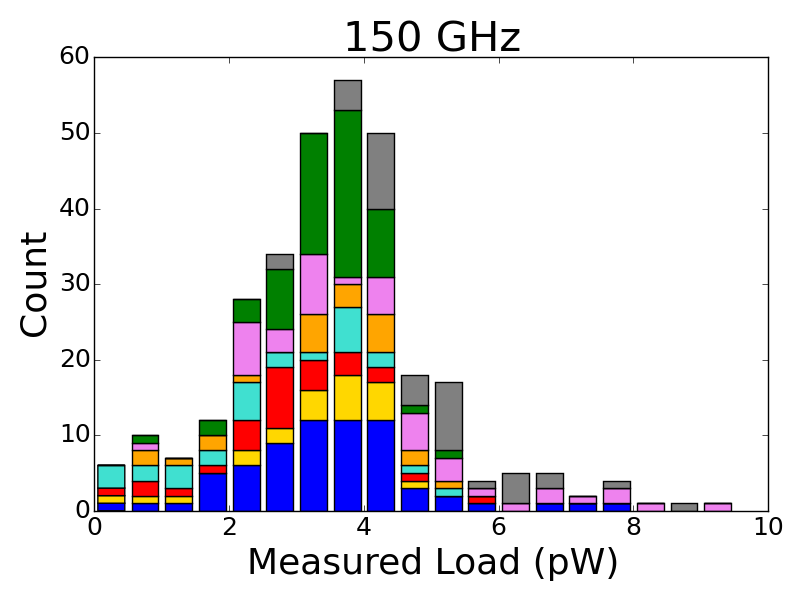
\includegraphics[width=0.32\columnwidth]{figures/ep2_150_radiative_load_hist}
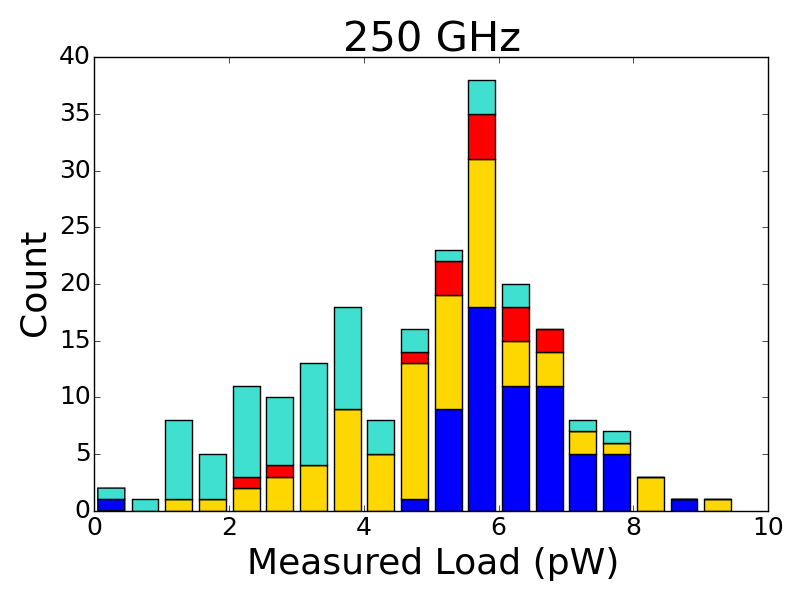
\includegraphics[width=0.32\columnwidth]{figures/ep2_250_radiative_load_hist}
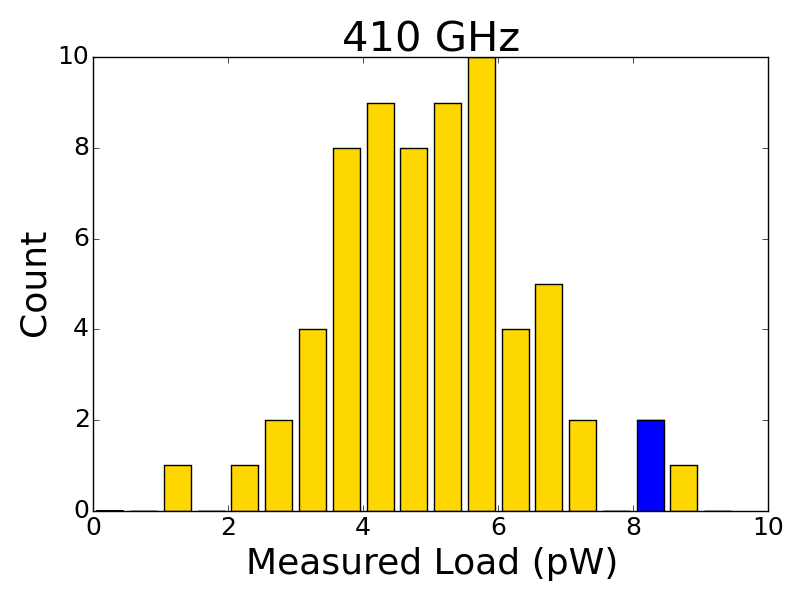
\includegraphics[width=0.32\columnwidth]{figures/ep2_410_radiative_load_hist}
%\end{tabular}
\caption{Histograms of the measured radiative load from the first detector tuning at float. The different colors represent 
different wafers.  The medians and standard deviations of the distributions are $3.6\pm 1.5, \, 5.3\pm 1.8$, and $5.0 \pm 1.4$~pW,
%gaussian fits were $3.6\pm 1.0, \, 5.3\pm 1.8$, and $4.9 \pm 1.4$~pW, - wow these agreed closely!
for the 150, 250, and 410~GHz, respectively. 
\label{fig:radiative_load_histograms} }
\end{center}
\end{figure}


%%%%%%%%%%%%%%%%%%%%%%%%%%%%%%%%%%%%%%%%%%%%%%%%%%%%%%%%%%%%%%%%%%%%%%%%%%%%%%}}}



%%%%%%%%%%%%%%%%%%%%%%%%%%%%%%%%%%%%%%%%%%%%%%%%%%%%%%%%%%%%%%%%%%%%%%%%%%%%%%%%
% Detector Flight Performance 
%%%%%%%%%%%%%%%%%%%%%%%%%%%%%%%%%%%%%%%%%%%%%%%%%%%%%%%%%%%%%%%%%%%%%%%%%%%%%%%%
\section{Noise Performance}
\label{sec:noise_performance}
%%%%%%%%%%%%%%%%%%%%%%%%%%%%%%%%%%%%%%%%%%%%%%%%%%%%%%%%%%%%%%%%%%%%%%%%%%%%%%%%

\begin{figure}[ht!]
\begin{center}
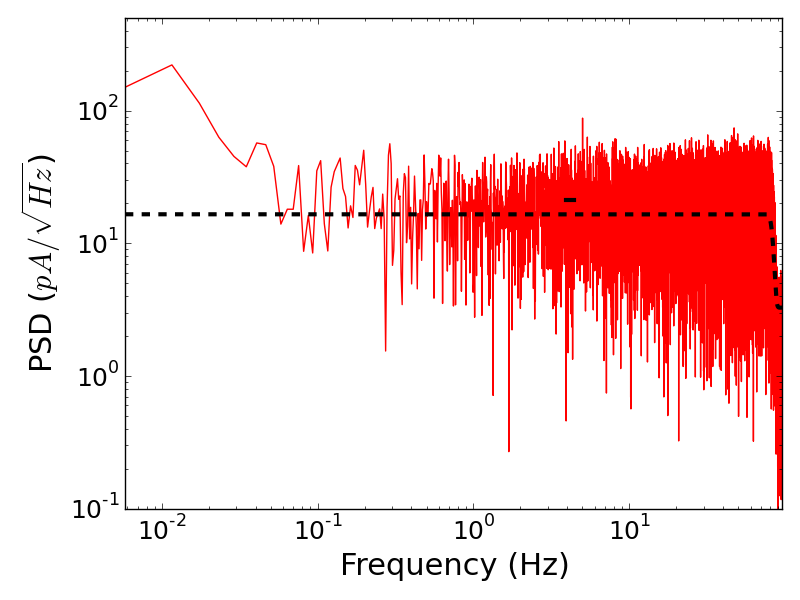
\includegraphics[width=0.48\columnwidth]{figures/board66_wire1_ch03_1356968507s_overbias}
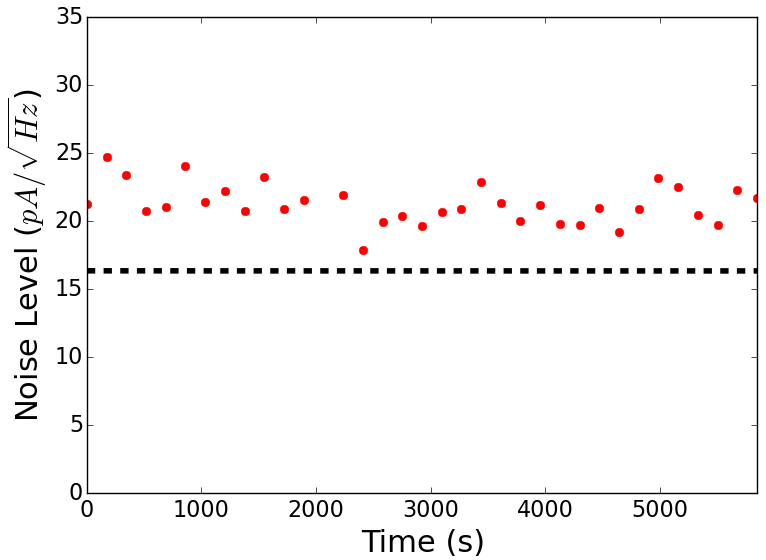
\includegraphics[width=0.48\columnwidth]{figures/board66_wire1_ch03_overbias}
\caption{Left: 
Right: . 
\label{fig:one_bolo_overbias_noise} }
\end{center}
\end{figure}

\begin{figure}[ht!]
\begin{center}
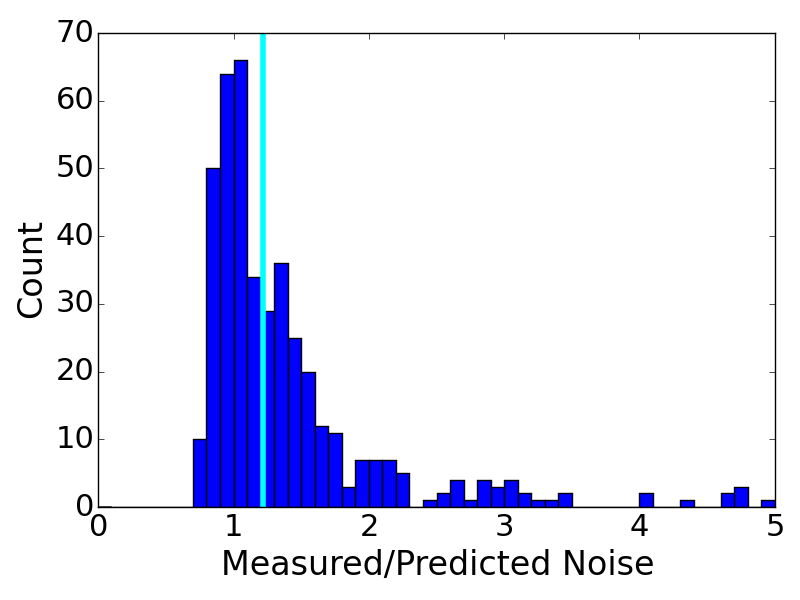
\includegraphics[height=2.5in]{figures/overbias_noise_ratios_histogram}
\caption{Histogram of the median ratio of measured to corrected predicted readout and Johnson noise for all bolometers. 
There are 34 bolometers with a ratio greater than 5.
The median value (vertical cyan) is 1.2. 
\label{fig:overbias_noise_hist} }
\end{center}
\end{figure}

\begin{table}[ht!]
\begin{center}
\begin{tabular}{| c | c | c |}
\hline  
           & Prediction           & Measured   \\
Wafer & (pA/$\sqrt{\mathrm{Hz}}$) & Ratio  \\
\hline 150-09 & 18 &  1.1 \\ 
\hline 150-14 & 17 &  1.1 \\ 
\hline 150-15 & 16 &  1.2 \\ 
%\hline 150-20 & Failed & Failed \\
%\hline 150-24 & 7.0 & 1.57 & Failed \\
\hline 150-39 & 19 &  1.5 \\ 
\hline 150-43 & 19 &  1.1 \\
\hline 150-47 & 21 &  1.1 \\
\hline 250-23 & 19 &  1.0 \\ 
\hline 250-24 & 21 &  1.3 \\ 
%\hline 250-25 & 1.94 & Failed \\
\hline 250-29 & 18 &  1.4 \\
%\hline 410-18 & 5.40 & Failed \\ 
\hline 410-28 & 24 &  1.4 \\
\hline
\end{tabular}
\end{center}
\caption{The predicted combination of Johnson and readout noise given each wafer's characterization measurements of $R_{N}$ and XXX. These predictions have been boosted by a factor of XXX, the excess of noise measured by the resistors. For each wafer the ratio quoted is  the median of the distribution for the detectors on that wafer. 
\label{tab:overbias_noise_table} }
\end{table}



\begin{figure}[ht!]
\begin{center}
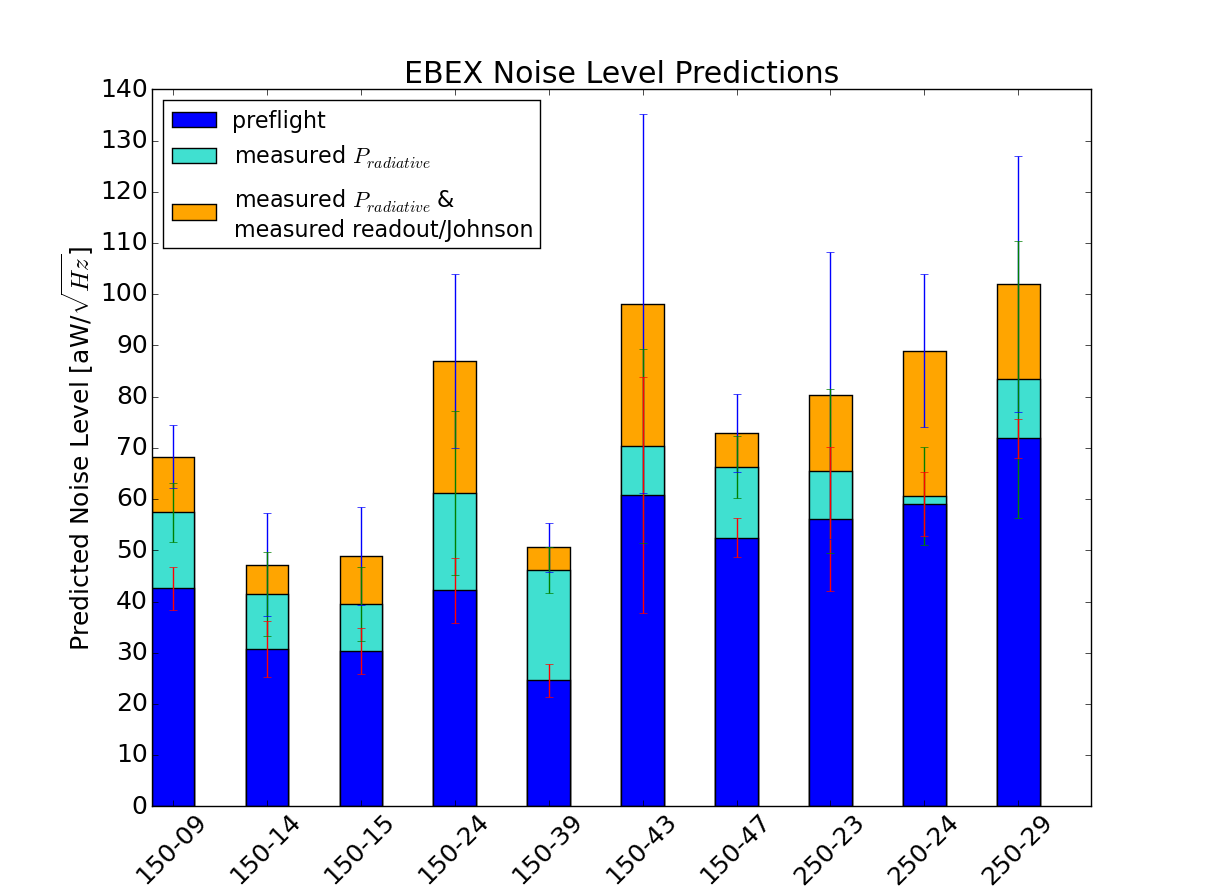
\includegraphics[height=2.5in]{figures/ebex_noise_level_predictions_barchart_per_wafer}
\caption{The \ac{EBEX} pre-flight \ac{NEP} prediction (blue), including the measured radiative load (cyan), and including the boost to readout and Johnson noise (gold).
\label{fig:prediction_bar_chart} }
\end{center}
\end{figure}

\begin{figure}[ht!]
  \begin{center}
    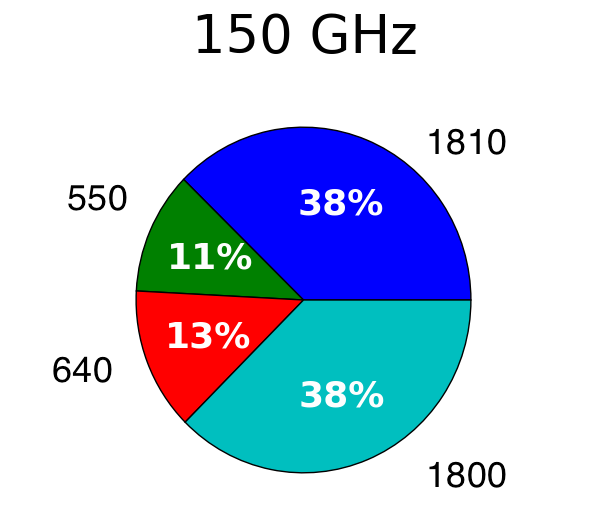
\includegraphics[width=0.29\columnwidth]{figures/150_average_noise_contribution_pie_chart.png}
    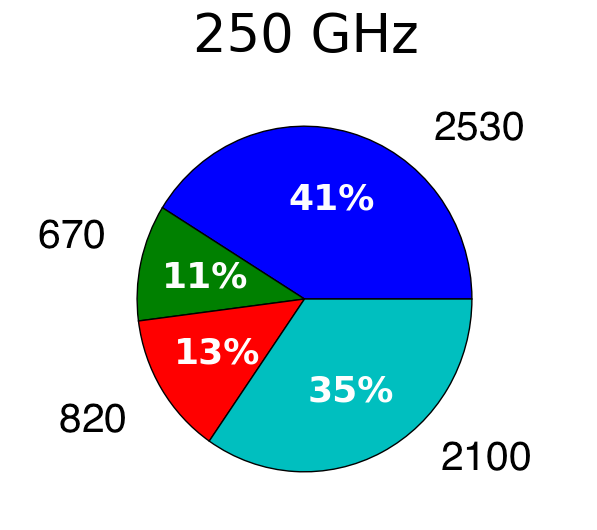
\includegraphics[width=0.29\columnwidth]{figures/250_average_noise_contribution_pie_chart.png}
    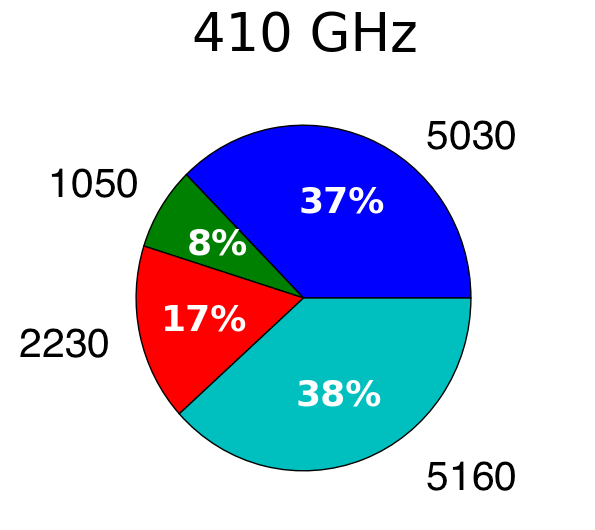
\includegraphics[width=0.29\columnwidth]{figures/410_average_noise_contribution_pie_chart.png}
    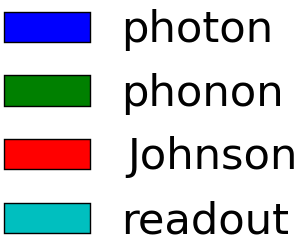
\includegraphics[width=0.1\columnwidth]{figures/piechart_legend.png}
    \caption{Individual components of the \ac{NEP} prediction in aW$^{2}$/Hz per band.
      The readout and Johnson \ac{NEP} terms include the excess factors measured with the resistors alone and with the bolometers biased above their superconducting transition.
      % We hypothesize that the excess readout noise is due to electromagnetic pickup.
      \label{fig:in_transition_pie} }
  \end{center}
\end{figure}

\begin{figure}[ht!]
\begin{center}
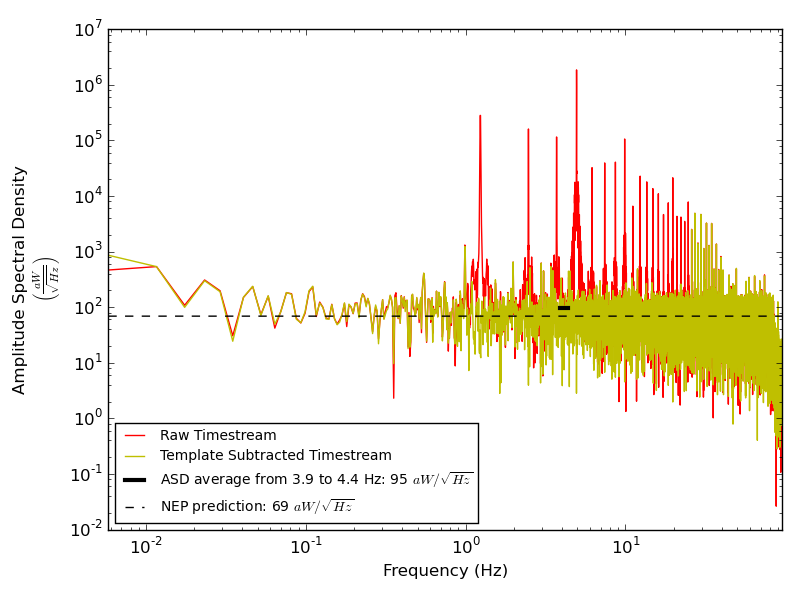
\includegraphics[height=2.5in]{figures/board68_wire2_ch04_1356979731s_transition.png}
\caption{In transition noise with the \ac{HWP} template present (red) and subtracted (gold).
\label{fig:one_bolo_overbias_noise} }
\end{center}
\end{figure}


\begin{figure}[ht!]
\begin{center}
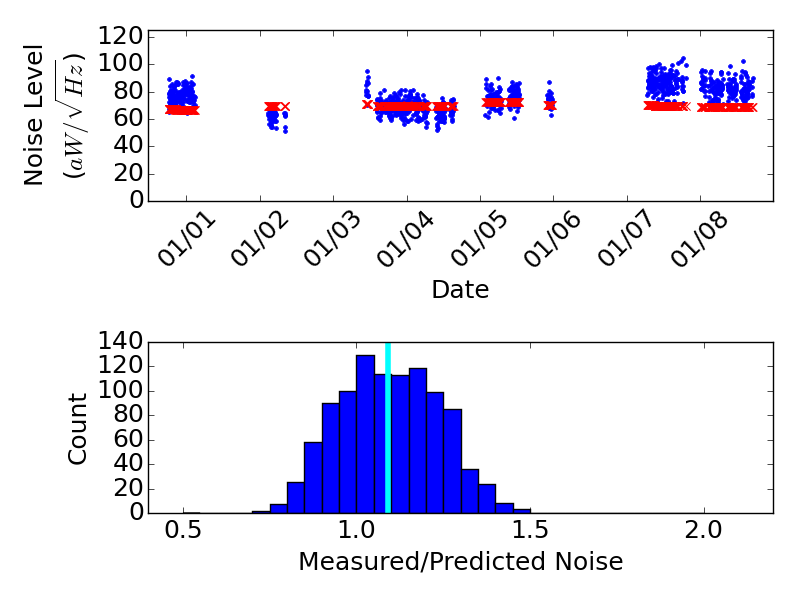
\includegraphics[width=0.48\columnwidth]{figures/board68_wire2_ch06_transition.png}
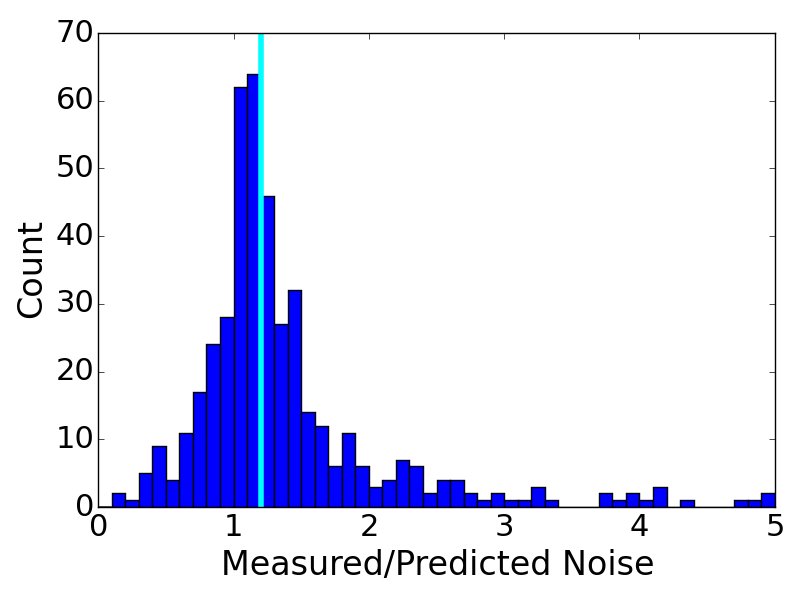
\includegraphics[width=0.48\columnwidth]{figures/in_transition_histogram.png}
\caption{Left top: in-transition measured (blue dots) and predicted corrected for excess noise above the transition (red crosses) \ac{NEP} for one 150~GHz detector 
throughout flight. Gaps indicate times that data is absent or rejected. 
Left bottom: distribution 
of measured-to-predicted ratio for this detector throughout flight, and the median (vertical cyan) ratio of 1.1.
Right: the distribution of the median ratio of measured to predicted in-transition noise corrected for excess noise above the transition throughout flight for all bolometers.
The median ratio (vertical cyan) is 1.2. 
\label{fig:in_transition_noise} }
\end{center}
\end{figure}



\begin{table}[ht!]
\begin{center}
\begin{tabular}{|c|c|c|c|}
\hline  Wafer & Predicted NEP [aW/$\sqrt{\mathrm{Hz}}$] & Measured/Predicted NEP \\
\hline 150-09 & 68 & 1.1 \\
\hline 150-14 & 45 & 0.8 \\
\hline 150-15 & 47 & 1.2 \\
%\hline 150-20 & n/a \\
%\hline 150-24 & n/a \\
\hline 150-39 & 77 & 1.1 \\
\hline 150-43 & 56 & 1.1 \\
\hline 150-47 & 59 & 1.4 \\
\hline 250-23 & 80 & 1.1 \\
\hline 250-24 & 76 & 1.4 \\
%\hline 250-25 & n/a \\
\hline 250-29 & 93 & 1.5 \\
%\hline 410-18 & n/a \\
\hline 
410-28 & 110 & 1.6 \\
\hline
All Detectors &  & 1.2 \\
\hline
\end{tabular}
\end{center}
\caption{The median predicted \ac{NEP} and measured-to-predicted ratio corrected for excess noise above the superconducting transition for each wafer and combined for 
all detectors.
}
\label{tab:in_transition_noise_table}
\end{table}





There is an increase of XXX when measuring the \ac{NEP} of the template subtracted data versus that measured from the "raw" timestream when the \ac{HWP} is still. 

\begin{figure}[ht!]
\begin{center}
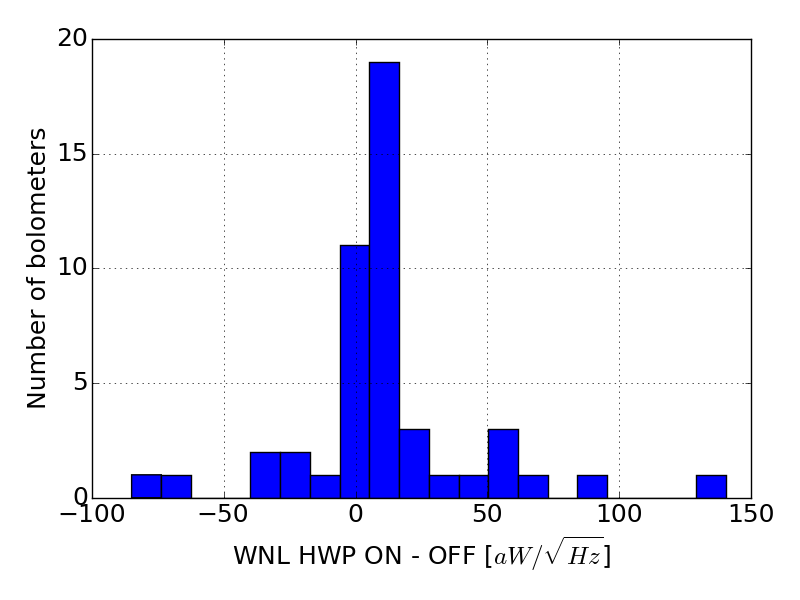
\includegraphics[width=0.45\columnwidth]{figures/hwp_on_and_off_median_diff_histogram}
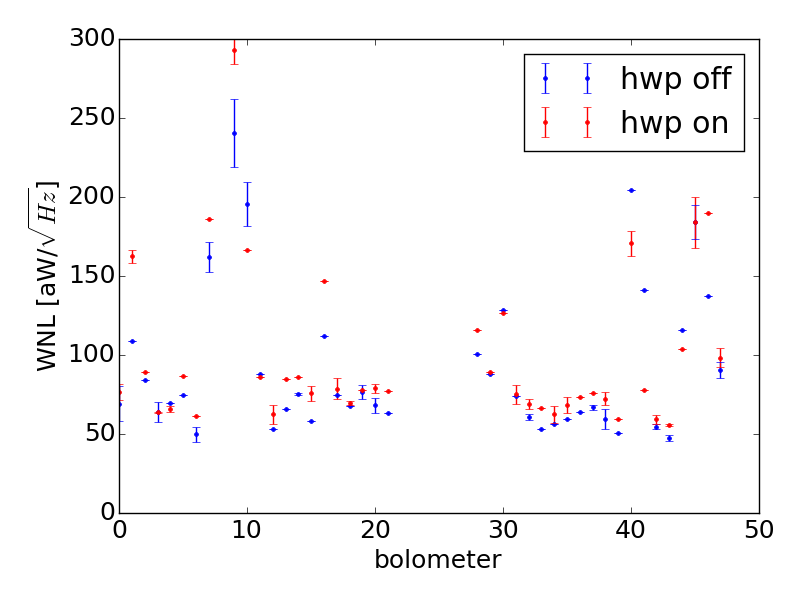
\includegraphics[width=0.45\columnwidth]{figures/hwp_on_and_off_cutoff_at_300aW}
\caption{Left: The difference of the \ac{NEP} measured with the \ac{HWP} on and off. Right: In-transition \ac{NEP} with the \ac{HWP} off (blue) and ten minutes later with the HWP on but subtracted (red). The error bars are the standard deviation of all the measurements over the ten minutes of data analyzed. If there is only one point, there are no error bars. 
\label{fig:hwp_on_vs_off} }
\end{center}
\end{figure}



%%%%%%%%%%%%%%%%%%%%%%%%%%%%%%%%%%%%%%%%%%%%%%%%%%%%%%%%%%%%%%%%%%%%%%%%%%%%%%}}}

